% Options for packages loaded elsewhere
\PassOptionsToPackage{unicode}{hyperref}
\PassOptionsToPackage{hyphens}{url}
%
\documentclass[
]{article}
\usepackage{lmodern}
\usepackage{amssymb,amsmath}
\usepackage{ifxetex,ifluatex}
\ifnum 0\ifxetex 1\fi\ifluatex 1\fi=0 % if pdftex
  \usepackage[T1]{fontenc}
  \usepackage[utf8]{inputenc}
  \usepackage{textcomp} % provide euro and other symbols
\else % if luatex or xetex
  \usepackage{unicode-math}
  \defaultfontfeatures{Scale=MatchLowercase}
  \defaultfontfeatures[\rmfamily]{Ligatures=TeX,Scale=1}
\fi
% Use upquote if available, for straight quotes in verbatim environments
\IfFileExists{upquote.sty}{\usepackage{upquote}}{}
\IfFileExists{microtype.sty}{% use microtype if available
  \usepackage[]{microtype}
  \UseMicrotypeSet[protrusion]{basicmath} % disable protrusion for tt fonts
}{}
\makeatletter
\@ifundefined{KOMAClassName}{% if non-KOMA class
  \IfFileExists{parskip.sty}{%
    \usepackage{parskip}
  }{% else
    \setlength{\parindent}{0pt}
    \setlength{\parskip}{6pt plus 2pt minus 1pt}}
}{% if KOMA class
  \KOMAoptions{parskip=half}}
\makeatother
\usepackage{xcolor}
\IfFileExists{xurl.sty}{\usepackage{xurl}}{} % add URL line breaks if available
\IfFileExists{bookmark.sty}{\usepackage{bookmark}}{\usepackage{hyperref}}
\hypersetup{
  pdftitle={CodeReport ST841 TAA Project},
  pdfauthor={Andrew Hollis, Xinyu Zhang, and Qiang Heng},
  hidelinks,
  pdfcreator={LaTeX via pandoc}}
\urlstyle{same} % disable monospaced font for URLs
\usepackage[margin=1in]{geometry}
\usepackage{color}
\usepackage{fancyvrb}
\newcommand{\VerbBar}{|}
\newcommand{\VERB}{\Verb[commandchars=\\\{\}]}
\DefineVerbatimEnvironment{Highlighting}{Verbatim}{commandchars=\\\{\}}
% Add ',fontsize=\small' for more characters per line
\usepackage{framed}
\definecolor{shadecolor}{RGB}{248,248,248}
\newenvironment{Shaded}{\begin{snugshade}}{\end{snugshade}}
\newcommand{\AlertTok}[1]{\textcolor[rgb]{0.94,0.16,0.16}{#1}}
\newcommand{\AnnotationTok}[1]{\textcolor[rgb]{0.56,0.35,0.01}{\textbf{\textit{#1}}}}
\newcommand{\AttributeTok}[1]{\textcolor[rgb]{0.77,0.63,0.00}{#1}}
\newcommand{\BaseNTok}[1]{\textcolor[rgb]{0.00,0.00,0.81}{#1}}
\newcommand{\BuiltInTok}[1]{#1}
\newcommand{\CharTok}[1]{\textcolor[rgb]{0.31,0.60,0.02}{#1}}
\newcommand{\CommentTok}[1]{\textcolor[rgb]{0.56,0.35,0.01}{\textit{#1}}}
\newcommand{\CommentVarTok}[1]{\textcolor[rgb]{0.56,0.35,0.01}{\textbf{\textit{#1}}}}
\newcommand{\ConstantTok}[1]{\textcolor[rgb]{0.00,0.00,0.00}{#1}}
\newcommand{\ControlFlowTok}[1]{\textcolor[rgb]{0.13,0.29,0.53}{\textbf{#1}}}
\newcommand{\DataTypeTok}[1]{\textcolor[rgb]{0.13,0.29,0.53}{#1}}
\newcommand{\DecValTok}[1]{\textcolor[rgb]{0.00,0.00,0.81}{#1}}
\newcommand{\DocumentationTok}[1]{\textcolor[rgb]{0.56,0.35,0.01}{\textbf{\textit{#1}}}}
\newcommand{\ErrorTok}[1]{\textcolor[rgb]{0.64,0.00,0.00}{\textbf{#1}}}
\newcommand{\ExtensionTok}[1]{#1}
\newcommand{\FloatTok}[1]{\textcolor[rgb]{0.00,0.00,0.81}{#1}}
\newcommand{\FunctionTok}[1]{\textcolor[rgb]{0.00,0.00,0.00}{#1}}
\newcommand{\ImportTok}[1]{#1}
\newcommand{\InformationTok}[1]{\textcolor[rgb]{0.56,0.35,0.01}{\textbf{\textit{#1}}}}
\newcommand{\KeywordTok}[1]{\textcolor[rgb]{0.13,0.29,0.53}{\textbf{#1}}}
\newcommand{\NormalTok}[1]{#1}
\newcommand{\OperatorTok}[1]{\textcolor[rgb]{0.81,0.36,0.00}{\textbf{#1}}}
\newcommand{\OtherTok}[1]{\textcolor[rgb]{0.56,0.35,0.01}{#1}}
\newcommand{\PreprocessorTok}[1]{\textcolor[rgb]{0.56,0.35,0.01}{\textit{#1}}}
\newcommand{\RegionMarkerTok}[1]{#1}
\newcommand{\SpecialCharTok}[1]{\textcolor[rgb]{0.00,0.00,0.00}{#1}}
\newcommand{\SpecialStringTok}[1]{\textcolor[rgb]{0.31,0.60,0.02}{#1}}
\newcommand{\StringTok}[1]{\textcolor[rgb]{0.31,0.60,0.02}{#1}}
\newcommand{\VariableTok}[1]{\textcolor[rgb]{0.00,0.00,0.00}{#1}}
\newcommand{\VerbatimStringTok}[1]{\textcolor[rgb]{0.31,0.60,0.02}{#1}}
\newcommand{\WarningTok}[1]{\textcolor[rgb]{0.56,0.35,0.01}{\textbf{\textit{#1}}}}
\usepackage{graphicx,grffile}
\makeatletter
\def\maxwidth{\ifdim\Gin@nat@width>\linewidth\linewidth\else\Gin@nat@width\fi}
\def\maxheight{\ifdim\Gin@nat@height>\textheight\textheight\else\Gin@nat@height\fi}
\makeatother
% Scale images if necessary, so that they will not overflow the page
% margins by default, and it is still possible to overwrite the defaults
% using explicit options in \includegraphics[width, height, ...]{}
\setkeys{Gin}{width=\maxwidth,height=\maxheight,keepaspectratio}
% Set default figure placement to htbp
\makeatletter
\def\fps@figure{htbp}
\makeatother
\setlength{\emergencystretch}{3em} % prevent overfull lines
\providecommand{\tightlist}{%
  \setlength{\itemsep}{0pt}\setlength{\parskip}{0pt}}
\setcounter{secnumdepth}{-\maxdimen} % remove section numbering

\title{CodeReport ST841 TAA Project}
\author{Andrew Hollis, Xinyu Zhang, and Qiang Heng}
\date{10/26/2020}

\begin{document}
\maketitle

\begin{Shaded}
\begin{Highlighting}[]
\NormalTok{knitr}\OperatorTok{::}\NormalTok{opts_chunk}\OperatorTok{$}\KeywordTok{set}\NormalTok{(}\DataTypeTok{echo =} \OtherTok{TRUE}\NormalTok{)}
\KeywordTok{library}\NormalTok{(knitr) }\CommentTok{# kable}
\KeywordTok{library}\NormalTok{(readr) }\CommentTok{# read_delim}
\KeywordTok{library}\NormalTok{(dplyr) }\CommentTok{# manipulate data}
\end{Highlighting}
\end{Shaded}

\begin{verbatim}
## 
## Attaching package: 'dplyr'
\end{verbatim}

\begin{verbatim}
## The following objects are masked from 'package:stats':
## 
##     filter, lag
\end{verbatim}

\begin{verbatim}
## The following objects are masked from 'package:base':
## 
##     intersect, setdiff, setequal, union
\end{verbatim}

\begin{Shaded}
\begin{Highlighting}[]
\KeywordTok{library}\NormalTok{(Amelia) }\CommentTok{# missing value imputation}
\end{Highlighting}
\end{Shaded}

\begin{verbatim}
## Loading required package: Rcpp
\end{verbatim}

\begin{verbatim}
## ## 
## ## Amelia II: Multiple Imputation
## ## (Version 1.7.6, built: 2019-11-24)
## ## Copyright (C) 2005-2020 James Honaker, Gary King and Matthew Blackwell
## ## Refer to http://gking.harvard.edu/amelia/ for more information
## ##
\end{verbatim}

\hypertarget{introduction}{%
\subsection{Introduction}\label{introduction}}

This document is meant to explain and demonstrate the implementation of
all analysis performed on the TAA dataset.

\hypertarget{data-transformations}{%
\subsection{Data Transformations}\label{data-transformations}}

We took the original data and performed several important
transformations.

First we read in the initial data file:

\begin{Shaded}
\begin{Highlighting}[]
\NormalTok{init_TAA_data<-}\KeywordTok{read.delim}\NormalTok{(}\StringTok{"initial_data.txt"}\NormalTok{)}
\NormalTok{init_TAA_data}\OperatorTok{$}\NormalTok{X3_firmSize <-}\StringTok{ }\KeywordTok{as.numeric}\NormalTok{(init_TAA_data}\OperatorTok{$}\NormalTok{Q26_num) }\CommentTok{# Insure Q26_num is actually numeric}
\NormalTok{init_TAA_data}\OperatorTok{$}\NormalTok{Q29_num<-}\KeywordTok{as.numeric}\NormalTok{(}\KeywordTok{as.character}\NormalTok{(init_TAA_data}\OperatorTok{$}\NormalTok{Q29_num)) }\CommentTok{#Insure Q29_num is actually numeric}
\end{Highlighting}
\end{Shaded}

\begin{verbatim}
## Warning: 强制改变过程中产生了NA
\end{verbatim}

\hypertarget{preview-the-missing-value}{%
\subsubsection{Preview the missing
value}\label{preview-the-missing-value}}

\begin{Shaded}
\begin{Highlighting}[]
\KeywordTok{missmap}\NormalTok{(init_TAA_data)}
\end{Highlighting}
\end{Shaded}

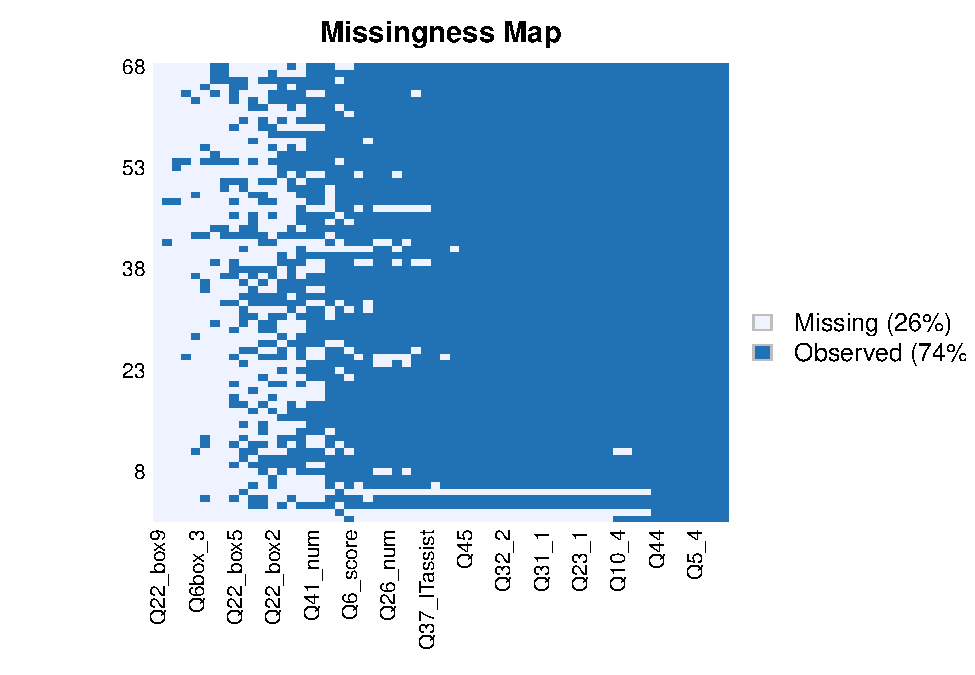
\includegraphics{markdown_report_files/figure-latex/unnamed-chunk-2-1.pdf}

The above plot shows how the missing value is distributed among the
data. The X-axis represent the variables that have missing value, and
the y-axis shows the observation.

For some observation such as 1, 2, and 5, we could see there are too
much missing values, thus it might need further consideration that if we
should include those data with most variables missing.

For the variables from left to right, the missing proportion for each
variable is decreasing, which need our further attention to select the
proper variable for analysis.

We then remove the variables that are not as interesting for analysis,
and these include the data from Q42, Q43, Q44, and Q45 which are
demographic data about the respondent. We will also compute new summary
score for question 6 from the survey, so we remove this as well.

\begin{Shaded}
\begin{Highlighting}[]
\NormalTok{removal_list<-}\KeywordTok{c}\NormalTok{(}\StringTok{"Q42"}\NormalTok{,}\StringTok{"Q43"}\NormalTok{,}\StringTok{"Q44"}\NormalTok{,}\StringTok{"Q45"}\NormalTok{,}\StringTok{"Q6_score"}\NormalTok{)}
\NormalTok{init_TAA_data<-init_TAA_data[, }\OperatorTok{!}\NormalTok{(}\KeywordTok{names}\NormalTok{(init_TAA_data) }\OperatorTok\NormalTok{removal_list)]}
\end{Highlighting}
\end{Shaded}

\hypertarget{dealing-with-likert-scale-items-drew}{%
\subsubsection{Dealing with Likert Scale Items
(Drew)}\label{dealing-with-likert-scale-items-drew}}

Questions 5, 10, 23, 30, 31, and 32 are composed of several 5-item
Likert scale sub-questions. Each of these questions represents a single
underlying conceptual variable. For instance, the 6 subquestions from
question 5 together measure the extent to which a business considered
various business objectives as they intially considered whether they
would try TAA tools. We would like to create a one-dimensional measure
that represents the level of this initial TAA consideration for a
particular company.

Nonlinear principal components analysis is a methodology that allows us
to transform several Likert scale items into the one-dimensional summary
metric that captures the maximal amount of variability from the original
data. (Linting et al. 2007)

Below, we use R to perform the nonlinear principal components analysis:

\begin{Shaded}
\begin{Highlighting}[]
\KeywordTok{library}\NormalTok{(Gifi)}
\CommentTok{##Q5}
\CommentTok{#Set Aside Data for initiation}
\NormalTok{init_data_names<-}\KeywordTok{c}\NormalTok{(}\StringTok{"Q5_1"}\NormalTok{,}\StringTok{"Q5_2"}\NormalTok{,}\StringTok{"Q5_3"}\NormalTok{,}\StringTok{"Q5_4"}\NormalTok{,}\StringTok{"Q5_5"}\NormalTok{,}\StringTok{"Q5_6"}\NormalTok{) }
\NormalTok{init_data<-init_TAA_data[init_data_names]}

\CommentTok{#Code Missing Values}
\NormalTok{init_data<-}\KeywordTok{apply}\NormalTok{(init_data,}\DecValTok{2}\NormalTok{,}\ControlFlowTok{function}\NormalTok{(x)\{}\KeywordTok{ifelse}\NormalTok{(x}\OperatorTok{==}\DecValTok{6}\NormalTok{,}\OtherTok{NA}\NormalTok{,x)\}) }

\CommentTok{#Impute, transform, do PCA}
\NormalTok{pca_init<-}\KeywordTok{princals}\NormalTok{(init_data,}\DataTypeTok{ndim=}\DecValTok{1}\NormalTok{,}\DataTypeTok{missing =} \StringTok{"a"}\NormalTok{,}\DataTypeTok{degrees=}\DecValTok{2}\NormalTok{)}
\NormalTok{init_score<-pca_init}\OperatorTok{$}\NormalTok{objectscores[,}\DecValTok{1}\NormalTok{]}

\CommentTok{##Q10}
\CommentTok{#Set Aside Data for routinization}
\NormalTok{rout_data_names<-}\KeywordTok{c}\NormalTok{(}\StringTok{"Q10_1"}\NormalTok{,}\StringTok{"Q10_2"}\NormalTok{,}\StringTok{"Q10_3"}\NormalTok{,}\StringTok{"Q10_4"}\NormalTok{) }
\NormalTok{rout_data<-init_TAA_data[rout_data_names]}

\CommentTok{#Code Missing Values}
\NormalTok{rout_data<-}\KeywordTok{apply}\NormalTok{(rout_data,}\DecValTok{2}\NormalTok{,}\ControlFlowTok{function}\NormalTok{(x)\{}\KeywordTok{ifelse}\NormalTok{(x}\OperatorTok{==}\DecValTok{6}\NormalTok{,}\OtherTok{NA}\NormalTok{,x)\}) }

\CommentTok{#Impute, transform, do PCA}
\NormalTok{pca_rout<-}\KeywordTok{princals}\NormalTok{(rout_data,}\DataTypeTok{ndim=}\DecValTok{1}\NormalTok{,}\DataTypeTok{missing =} \StringTok{"a"}\NormalTok{,}\DataTypeTok{degrees=}\DecValTok{2}\NormalTok{)}
\NormalTok{rout_score<-pca_rout}\OperatorTok{$}\NormalTok{objectscores[,}\DecValTok{1}\NormalTok{]}

\CommentTok{##Q23}
\CommentTok{#Set Aside Data for routinization}
\NormalTok{integ_data_names<-}\KeywordTok{c}\NormalTok{(}\StringTok{"Q23_1"}\NormalTok{,}\StringTok{"Q23_2"}\NormalTok{) }
\NormalTok{integ_data<-init_TAA_data[integ_data_names]}

\CommentTok{#Code Missing Values}
\NormalTok{integ_data<-}\KeywordTok{apply}\NormalTok{(integ_data,}\DecValTok{2}\NormalTok{,}\ControlFlowTok{function}\NormalTok{(x)\{}\KeywordTok{ifelse}\NormalTok{(x}\OperatorTok{==}\DecValTok{6}\NormalTok{,}\OtherTok{NA}\NormalTok{,x)\}) }

\CommentTok{#Impute, transform, do PCA}
\NormalTok{pca_integ<-}\KeywordTok{princals}\NormalTok{(integ_data,}\DataTypeTok{ndim=}\DecValTok{1}\NormalTok{,}\DataTypeTok{missing =} \StringTok{"a"}\NormalTok{,}\DataTypeTok{degrees=}\DecValTok{2}\NormalTok{)}
\NormalTok{integ_score<-pca_integ}\OperatorTok{$}\NormalTok{objectscores[,}\DecValTok{1}\NormalTok{]}

\CommentTok{##Q30}
\CommentTok{#Set Aside Data for management obstacles}
\NormalTok{manag_data_names<-}\KeywordTok{c}\NormalTok{(}\StringTok{"Q30_1"}\NormalTok{,}\StringTok{"Q30_2"}\NormalTok{,}\StringTok{"Q30_3"}\NormalTok{,}\StringTok{"Q30_4"}\NormalTok{) }
\NormalTok{manag_data<-init_TAA_data[manag_data_names]}

\CommentTok{#Code Missing Values}
\NormalTok{manag_data<-}\KeywordTok{apply}\NormalTok{(manag_data,}\DecValTok{2}\NormalTok{,}\ControlFlowTok{function}\NormalTok{(x)\{}\KeywordTok{ifelse}\NormalTok{(x}\OperatorTok{==}\DecValTok{6}\NormalTok{,}\OtherTok{NA}\NormalTok{,x)\}) }

\CommentTok{#Impute, transform, do PCA}
\NormalTok{pca_manag<-}\KeywordTok{princals}\NormalTok{(manag_data,}\DataTypeTok{ndim=}\DecValTok{1}\NormalTok{,}\DataTypeTok{missing =} \StringTok{"a"}\NormalTok{,}\DataTypeTok{degrees=}\DecValTok{2}\NormalTok{)}
\NormalTok{manag_score<-pca_manag}\OperatorTok{$}\NormalTok{objectscores[,}\DecValTok{1}\NormalTok{]}

\CommentTok{##Q31}
\CommentTok{#Set Aside Data for management obstacles}
\NormalTok{comp_data_names<-}\KeywordTok{c}\NormalTok{(}\StringTok{"Q31_1"}\NormalTok{,}\StringTok{"Q31_2"}\NormalTok{,}\StringTok{"Q31_3"}\NormalTok{) }
\NormalTok{comp_data<-init_TAA_data[comp_data_names]}

\CommentTok{#Code Missing Values}
\NormalTok{comp_data<-}\KeywordTok{apply}\NormalTok{(comp_data,}\DecValTok{2}\NormalTok{,}\ControlFlowTok{function}\NormalTok{(x)\{}\KeywordTok{ifelse}\NormalTok{(x}\OperatorTok{==}\DecValTok{6}\NormalTok{,}\OtherTok{NA}\NormalTok{,x)\}) }

\CommentTok{#Impute, transform, do PCA}
\NormalTok{pca_comp<-}\KeywordTok{princals}\NormalTok{(comp_data,}\DataTypeTok{ndim=}\DecValTok{1}\NormalTok{,}\DataTypeTok{missing =} \StringTok{"a"}\NormalTok{,}\DataTypeTok{degrees=}\DecValTok{2}\NormalTok{)}
\NormalTok{comp_score<-pca_comp}\OperatorTok{$}\NormalTok{objectscores[,}\DecValTok{1}\NormalTok{]}

\CommentTok{##Q32}
\CommentTok{#Set Aside Data for Government Regulation}
\NormalTok{gov_data_names<-}\KeywordTok{c}\NormalTok{(}\StringTok{"Q32_1"}\NormalTok{,}\StringTok{"Q32_2"}\NormalTok{,}\StringTok{"Q32_3"}\NormalTok{,}\StringTok{"Q32_4"}\NormalTok{) }
\NormalTok{gov_data<-init_TAA_data[gov_data_names]}

\CommentTok{#Code Missing Values}
\NormalTok{gov_data<-}\KeywordTok{apply}\NormalTok{(gov_data,}\DecValTok{2}\NormalTok{,}\ControlFlowTok{function}\NormalTok{(x)\{}\KeywordTok{ifelse}\NormalTok{(x}\OperatorTok{==}\DecValTok{6}\NormalTok{,}\OtherTok{NA}\NormalTok{,x)\}) }

\CommentTok{#Impute, transform, do PCA}
\NormalTok{pca_gov<-}\KeywordTok{princals}\NormalTok{(gov_data,}\DataTypeTok{ndim=}\DecValTok{1}\NormalTok{,}\DataTypeTok{missing =} \StringTok{"a"}\NormalTok{,}\DataTypeTok{degrees=}\DecValTok{2}\NormalTok{)}
\NormalTok{gov_score<-pca_gov}\OperatorTok{$}\NormalTok{objectscores[,}\DecValTok{1}\NormalTok{]}

\CommentTok{#Add Nonlinear PCA Scores to data}
\NormalTok{init_TAA_data}\OperatorTok{$}\NormalTok{init_composite<-init_score}
\NormalTok{init_TAA_data}\OperatorTok{$}\NormalTok{rout_composite<-rout_score}
\NormalTok{init_TAA_data}\OperatorTok{$}\NormalTok{integrate_composite<-integ_score}
\NormalTok{init_TAA_data}\OperatorTok{$}\NormalTok{manag_composite<-manag_score}
\NormalTok{init_TAA_data}\OperatorTok{$}\NormalTok{comp_composite<-comp_score}
\NormalTok{init_TAA_data}\OperatorTok{$}\NormalTok{gov_composite<-gov_score}
\KeywordTok{str}\NormalTok{(init_TAA_data)}
\end{Highlighting}
\end{Shaded}

\begin{verbatim}
## 'data.frame':    68 obs. of  61 variables:
##  $ Q5_1               : int  6 1 4 5 5 4 3 3 3 4 ...
##  $ Q5_2               : int  6 5 4 5 2 1 1 4 4 3 ...
##  $ Q5_3               : int  6 5 4 4 3 3 5 4 4 4 ...
##  $ Q5_4               : int  6 5 5 5 5 5 5 5 4 4 ...
##  $ Q5_5               : int  6 5 5 4 5 5 5 5 3 5 ...
##  $ Q5_6               : int  6 5 5 5 5 5 5 5 5 5 ...
##  $ Q6box_1            : int  NA NA 1 NA 1 1 1 NA 1 1 ...
##  $ Q6box_2            : int  NA NA NA 2 2 NA NA NA NA 2 ...
##  $ Q6box_3            : int  NA NA NA NA NA NA 3 NA NA NA ...
##  $ Q6box_4            : int  NA 4 4 4 NA 4 NA NA NA NA ...
##  $ Q10_1              : int  2 3 3 3 3 3 5 3 3 3 ...
##  $ Q10_2              : int  2 3 3 3 3 3 4 3 3 3 ...
##  $ Q10_3              : int  1 1 3 2 1 1 3 1 1 2 ...
##  $ Q10_4              : int  1 1 3 2 1 1 3 1 1 2 ...
##  $ Q35_ERP            : int  1 1 1 1 1 1 1 0 0 1 ...
##  $ Q40_TAA            : int  0 1 1 1 1 1 1 0 0 0 ...
##  $ Q36_ITcount        : int  3 2 3 3 NA 3 0 2 2 3 ...
##  $ Q37_ITassist       : int  1 0 3 0 1 1 2 1 1 3 ...
##  $ Q38_Taxcount       : int  23 23 40 12 100 200 55 19 15 45 ...
##  $ Q39_TAAexpert      : num  1 2.5 10 2 2 40 2 1 4 3 ...
##  $ Q22_box1           : int  1 1 1 1 1 1 1 1 1 1 ...
##  $ Q22_box2           : int  NA 2 2 NA 2 2 NA NA NA 2 ...
##  $ Q22_box3           : int  3 NA 3 NA 3 3 3 NA NA NA ...
##  $ Q22_box4           : int  4 4 4 NA NA NA NA NA NA NA ...
##  $ Q22_box5           : int  NA NA 5 5 5 5 NA NA NA 5 ...
##  $ Q22_box6           : int  NA NA NA 6 NA NA NA NA NA NA ...
##  $ Q22_box7           : int  NA NA 7 NA NA NA 7 NA 7 7 ...
##  $ Q22_box8           : int  NA NA NA NA NA NA NA NA NA NA ...
##  $ Q22_box9           : logi  NA NA NA NA NA NA ...
##  $ Q22_box10          : int  NA NA NA NA 10 NA NA NA NA NA ...
##  $ Q23_1              : int  4 3 3 1 2 3 4 2 3 2 ...
##  $ Q23_2              : int  4 3 3 1 1 2 4 1 1 2 ...
##  $ Q26                : int  6 6 6 6 6 6 6 6 6 6 ...
##  $ Q24_box1           : int  NA NA NA NA NA NA NA NA NA NA ...
##  $ Q24_box2           : int  NA NA 2 2 2 2 NA NA 2 NA ...
##  $ Q24_box3           : int  NA NA 3 3 3 3 NA NA 3 NA ...
##  $ Q24_box4           : int  4 4 4 4 4 4 4 4 4 4 ...
##  $ Q27                : int  2 2 3 3 3 3 3 2 3 3 ...
##  $ Q29                : int  1 1 4 6 6 4 3 2 2 6 ...
##  $ Q41                : int  1 1 3 6 NA 4 1 2 2 NA ...
##  $ Q30_1              : int  5 1 3 4 4 3 1 4 4 3 ...
##  $ Q30_2              : int  4 1 2 2 3 3 1 5 3 3 ...
##  $ Q30_3              : int  4 3 2 4 5 4 1 3 5 3 ...
##  $ Q30_4              : int  NA NA NA NA NA 4 5 NA NA NA ...
##  $ Q31_1              : int  3 5 3 4 1 3 5 1 2 3 ...
##  $ Q31_2              : int  5 1 4 4 4 3 5 4 5 3 ...
##  $ Q31_3              : int  1 5 3 4 4 3 5 4 5 3 ...
##  $ Q32_1              : int  2 1 4 4 5 3 3 4 5 5 ...
##  $ Q32_2              : int  6 1 4 4 5 2 1 4 5 3 ...
##  $ Q32_3              : int  3 1 5 3 5 3 1 5 5 3 ...
##  $ Q32_4              : int  6 1 5 3 5 1 3 4 3 6 ...
##  $ Q26_num            : int  115000 9000 25000 28000 90000 60000 15000 5600 26000 70000 ...
##  $ Q29_num            : num  0 0.02 0.33 0.58 0.67 0.3 0.2 0.14 0.08 0.55 ...
##  $ Q41_num            : num  0 0 0.25 0.65 NA 0.3 0.01 0.1 0.08 NA ...
##  $ X3_firmSize        : num  115000 9000 25000 28000 90000 60000 15000 5600 26000 70000 ...
##  $ init_composite     : num  -1.5414 0.0756 0.5785 0.6462 0.3255 ...
##  $ rout_composite     : num  -0.9368 -0.9235 0.0819 -0.038 -0.9235 ...
##  $ integrate_composite: num  2.379 -0.182 -0.182 -0.758 -0.758 ...
##  $ manag_composite    : num  -0.864 2.7594 0.0495 -0.4805 -0.4805 ...
##  $ comp_composite     : num  -0.0581 0.9617 -0.9414 -0.9414 -0.9414 ...
##  $ gov_composite      : num  -0.197 -2.954 1.633 0.753 1.633 ...
\end{verbatim}

\begin{Shaded}
\begin{Highlighting}[]
\CommentTok{#Create Loadings Plots}
\KeywordTok{par}\NormalTok{(}\DataTypeTok{mfrow=}\KeywordTok{c}\NormalTok{(}\DecValTok{2}\NormalTok{,}\DecValTok{3}\NormalTok{))}
\KeywordTok{barplot}\NormalTok{(pca_init}\OperatorTok{$}\NormalTok{loadings[,}\DecValTok{1}\NormalTok{],}\DataTypeTok{main=}\StringTok{"Initiation Composite"}\NormalTok{)}
\KeywordTok{barplot}\NormalTok{(pca_rout}\OperatorTok{$}\NormalTok{loadings[,}\DecValTok{1}\NormalTok{],}\DataTypeTok{main=}\StringTok{"Routinization Composite"}\NormalTok{)}
\KeywordTok{barplot}\NormalTok{(pca_integ}\OperatorTok{$}\NormalTok{loadings[,}\DecValTok{1}\NormalTok{],}\DataTypeTok{main=}\StringTok{"Tech Integration Composite"}\NormalTok{)}
\KeywordTok{barplot}\NormalTok{(pca_manag}\OperatorTok{$}\NormalTok{loadings[,}\DecValTok{1}\NormalTok{],}\DataTypeTok{main=}\StringTok{"Management Obstacles Composite"}\NormalTok{)}
\KeywordTok{barplot}\NormalTok{(pca_comp}\OperatorTok{$}\NormalTok{loadings[,}\DecValTok{1}\NormalTok{],}\DataTypeTok{main=}\StringTok{"Competition Composite"}\NormalTok{)}
\KeywordTok{barplot}\NormalTok{(pca_gov}\OperatorTok{$}\NormalTok{loadings[,}\DecValTok{1}\NormalTok{],}\DataTypeTok{main=}\StringTok{"Regulatory Environment Composite"}\NormalTok{)}
\end{Highlighting}
\end{Shaded}

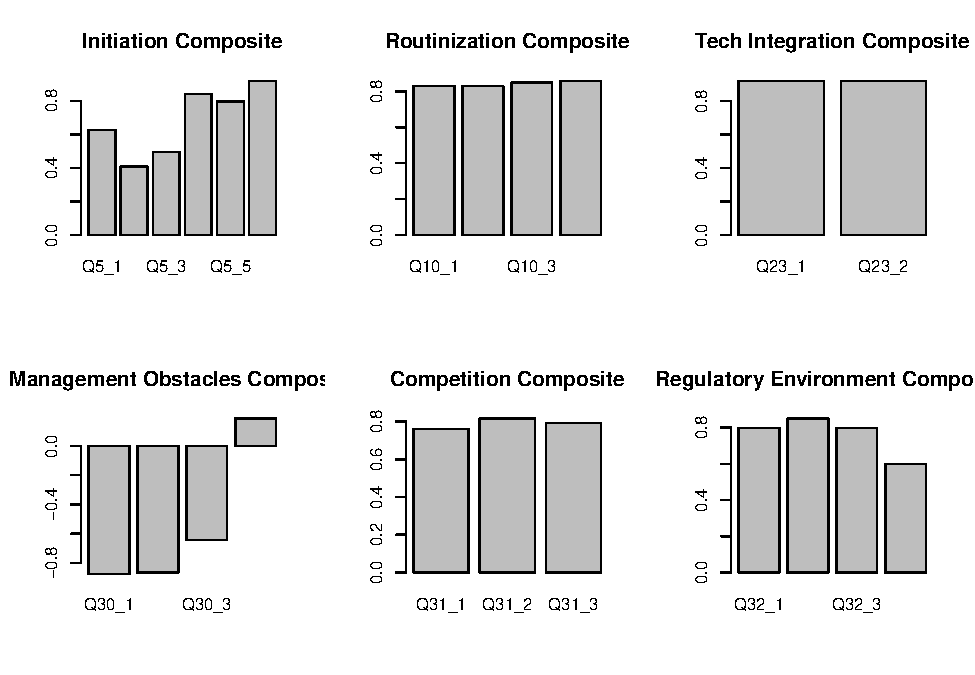
\includegraphics{markdown_report_files/figure-latex/unnamed-chunk-5-1.pdf}

\begin{Shaded}
\begin{Highlighting}[]
\CommentTok{#Remove Original Likert Scale Data}
\NormalTok{removal_list<-}\KeywordTok{c}\NormalTok{(}\StringTok{"Q5_1"}\NormalTok{,}\StringTok{"Q5_2"}\NormalTok{,}\StringTok{"Q5_3"}\NormalTok{,}\StringTok{"Q5_4"}\NormalTok{,}\StringTok{"Q5_5"}\NormalTok{,}\StringTok{"Q5_6"}\NormalTok{,}\StringTok{"Q10_1"}\NormalTok{,}\StringTok{"Q10_2"}\NormalTok{,}\StringTok{"Q10_3"}\NormalTok{,}\StringTok{"Q10_4"}\NormalTok{,}\StringTok{"Q23_1"}\NormalTok{,}\StringTok{"Q23_2"}\NormalTok{,}\StringTok{"Q30_1"}\NormalTok{,}\StringTok{"Q30_2"}\NormalTok{,}\StringTok{"Q30_3"}\NormalTok{,}\StringTok{"Q30_4"}\NormalTok{,}\StringTok{"Q31_1"}\NormalTok{,}\StringTok{"Q31_2"}\NormalTok{,}\StringTok{"Q31_3"}\NormalTok{,}\StringTok{"Q32_1"}\NormalTok{,}\StringTok{"Q32_2"}\NormalTok{,}\StringTok{"Q32_3"}\NormalTok{,}\StringTok{"Q32_4"}\NormalTok{)}
\NormalTok{init_TAA_data<-init_TAA_data[, }\OperatorTok{!}\NormalTok{(}\KeywordTok{names}\NormalTok{(init_TAA_data) }\OperatorTok\NormalTok{removal_list)]}
\end{Highlighting}
\end{Shaded}

\hypertarget{combining-weighted-variables-drew}{%
\subsubsection{Combining Weighted Variables
(Drew)}\label{combining-weighted-variables-drew}}

Q6 and Q22 have survey respondents check several boxes to indicate the
level of TAA technology they have adopted and the specific types of TAA
they adopted. For Q6, if respondents check the first box, they have
adopted emerging TAA technology, if they check the second box they have
adopted intermediate TAA technology, and if they check the third box
they have adopted advanced TAA technology. We assign a weight of 1 to
checkbox 1, 2 to checkbox 2, and 3 to checkbox 3. We create the single
adoption score for each company by adding the weights and dividing by
the maximum possible cumulative weight, 6.

Similarly, for Q22, if a weight of 0 is assigned to the first box, 1 to
the second box, 2 for the 3rd, 4th, 5th, and 10th boxes, 3 for the 6th
box, 4 for the 7th box, and 5 for the 8th and 9th boxes. As with the Q6
response, we form a single score by adding the weights and dividing by
the maximum potential score, 26.

We standardize both new scores to have zero meana and standard deviation
of 1.

We carry out this weighting in R below:

\begin{Shaded}
\begin{Highlighting}[]
\CommentTok{#Transform 4's}
\NormalTok{init_TAA_data[}\DecValTok{2}\NormalTok{,}\DecValTok{9}\NormalTok{]=}\DecValTok{3}
\NormalTok{init_TAA_data[}\DecValTok{16}\NormalTok{,}\DecValTok{7}\NormalTok{]=}\DecValTok{1}

\CommentTok{#Form Adoption Score}
\NormalTok{adopt_data<-init_TAA_data[}\KeywordTok{c}\NormalTok{(}\StringTok{"Q6box_1"}\NormalTok{,}\StringTok{"Q6box_2"}\NormalTok{,}\StringTok{"Q6box_3"}\NormalTok{)]}
\NormalTok{adopt_comp<-}\KeywordTok{apply}\NormalTok{(adopt_data,}\DecValTok{1}\NormalTok{,sum,}\DataTypeTok{na.rm=}\OtherTok{TRUE}\NormalTok{)}\OperatorTok{/}\DecValTok{6}
\NormalTok{init_TAA_data}\OperatorTok{$}\NormalTok{adoption_score<-adopt_comp}
\NormalTok{init_TAA_data}\OperatorTok{$}\NormalTok{adoption_score<-}\KeywordTok{scale}\NormalTok{(init_TAA_data}\OperatorTok{$}\NormalTok{adoption_score)}

\CommentTok{#Technology Readiness/Capability Score}
\NormalTok{TAA_capability_data<-init_TAA_data[}\KeywordTok{c}\NormalTok{(}\StringTok{"Q22_box1"}\NormalTok{,}\StringTok{"Q22_box2"}\NormalTok{,}\StringTok{"Q22_box3"}\NormalTok{,}\StringTok{"Q22_box4"}\NormalTok{,}\StringTok{"Q22_box5"}\NormalTok{,}\StringTok{"Q22_box6"}\NormalTok{,}\StringTok{"Q22_box7"}\NormalTok{,}\StringTok{"Q22_box8"}\NormalTok{,}\StringTok{"Q22_box9"}\NormalTok{, }\StringTok{"Q22_box10"}\NormalTok{)]}

\NormalTok{TAA_capability_score<-}\KeywordTok{rep}\NormalTok{(}\DecValTok{0}\NormalTok{,}\KeywordTok{nrow}\NormalTok{(TAA_capability_data))}
\NormalTok{max_score=}\DecValTok{1}\OperatorTok{+}\DecValTok{2}\OperatorTok{*}\DecValTok{4}\OperatorTok{+}\DecValTok{3}\OperatorTok{+}\DecValTok{4}\OperatorTok{+}\DecValTok{5}\OperatorTok{*}\DecValTok{2}
\ControlFlowTok{for}\NormalTok{(i }\ControlFlowTok{in} \DecValTok{1}\OperatorTok{:}\KeywordTok{length}\NormalTok{(TAA_capability_score))\{}
\NormalTok{  score=}\DecValTok{0}
  \ControlFlowTok{if}\NormalTok{(}\OperatorTok{!}\KeywordTok{is.na}\NormalTok{(TAA_capability_data[i,}\DecValTok{1}\NormalTok{]))\{}
\NormalTok{    score=score}\OperatorTok{+}\DecValTok{0}
\NormalTok{  \}}
  \ControlFlowTok{if}\NormalTok{(}\OperatorTok{!}\KeywordTok{is.na}\NormalTok{(TAA_capability_data[i,}\DecValTok{2}\NormalTok{]))\{}
\NormalTok{    score=score}\OperatorTok{+}\DecValTok{1}
\NormalTok{  \}}
  \ControlFlowTok{if}\NormalTok{(}\OperatorTok{!}\KeywordTok{is.na}\NormalTok{(TAA_capability_data[i,}\DecValTok{3}\NormalTok{]))\{}
\NormalTok{    score=score}\OperatorTok{+}\DecValTok{2}
\NormalTok{  \}}
  \ControlFlowTok{if}\NormalTok{(}\OperatorTok{!}\KeywordTok{is.na}\NormalTok{(TAA_capability_data[i,}\DecValTok{4}\NormalTok{]))\{}
\NormalTok{    score=score}\OperatorTok{+}\DecValTok{2}
\NormalTok{  \}}
  \ControlFlowTok{if}\NormalTok{(}\OperatorTok{!}\KeywordTok{is.na}\NormalTok{(TAA_capability_data[i,}\DecValTok{5}\NormalTok{]))\{}
\NormalTok{    score=score}\OperatorTok{+}\DecValTok{2}
\NormalTok{  \}}
  \ControlFlowTok{if}\NormalTok{(}\OperatorTok{!}\KeywordTok{is.na}\NormalTok{(TAA_capability_data[i,}\DecValTok{6}\NormalTok{]))\{}
\NormalTok{    score=score}\OperatorTok{+}\DecValTok{3}
\NormalTok{  \}}
  \ControlFlowTok{if}\NormalTok{(}\OperatorTok{!}\KeywordTok{is.na}\NormalTok{(TAA_capability_data[i,}\DecValTok{7}\NormalTok{]))\{}
\NormalTok{    score=score}\OperatorTok{+}\DecValTok{4}
\NormalTok{  \}}
  \ControlFlowTok{if}\NormalTok{(}\OperatorTok{!}\KeywordTok{is.na}\NormalTok{(TAA_capability_data[i,}\DecValTok{8}\NormalTok{]))\{}
\NormalTok{    score=score}\OperatorTok{+}\DecValTok{5}
\NormalTok{  \}}
  \ControlFlowTok{if}\NormalTok{(}\OperatorTok{!}\KeywordTok{is.na}\NormalTok{(TAA_capability_data[i,}\DecValTok{9}\NormalTok{]))\{}
\NormalTok{    score=score}\OperatorTok{+}\DecValTok{5}
\NormalTok{  \}}
  \ControlFlowTok{if}\NormalTok{(}\OperatorTok{!}\KeywordTok{is.na}\NormalTok{(TAA_capability_data[i,}\DecValTok{10}\NormalTok{]))\{}
\NormalTok{    score=score}\OperatorTok{+}\DecValTok{2}
\NormalTok{  \}}
\NormalTok{  TAA_capability_score[i]=score}\OperatorTok{/}\NormalTok{max_score}
\NormalTok{\}}
\NormalTok{init_TAA_data}\OperatorTok{$}\NormalTok{TAA_capability<-TAA_capability_score}
\NormalTok{init_TAA_data}\OperatorTok{$}\NormalTok{TAA_capability<-}\KeywordTok{scale}\NormalTok{(init_TAA_data}\OperatorTok{$}\NormalTok{TAA_capability)}
\end{Highlighting}
\end{Shaded}

\hypertarget{creating-binary-variable-for-q24}{%
\subsubsection{Creating Binary Variable for
Q24}\label{creating-binary-variable-for-q24}}

Q24 measures the global extent of a company. We transform this variable
into a binary variable that is 0 if the company only has domestic
offices and 1 if the company has foreign offices.

\begin{Shaded}
\begin{Highlighting}[]
\NormalTok{dom_int_data<-init_TAA_data[}\KeywordTok{c}\NormalTok{(}\StringTok{"Q24_box1"}\NormalTok{,}\StringTok{"Q24_box2"}\NormalTok{,}\StringTok{"Q24_box3"}\NormalTok{,}\StringTok{"Q24_box4"}\NormalTok{)]}
\NormalTok{dom_int<-}\KeywordTok{ifelse}\NormalTok{(}\KeywordTok{is.na}\NormalTok{(dom_int_data[,}\DecValTok{4}\NormalTok{]),}\DecValTok{0}\NormalTok{,}\DecValTok{1}\NormalTok{) }\CommentTok{#Create binary variable}
\NormalTok{init_TAA_data}\OperatorTok{$}\NormalTok{Domestic_International<-dom_int}
\NormalTok{NA_index=}\KeywordTok{apply}\NormalTok{(}\KeywordTok{is.na}\NormalTok{(init_TAA_data[}\KeywordTok{c}\NormalTok{(}\StringTok{"Q24_box1"}\NormalTok{,}\StringTok{"Q24_box2"}\NormalTok{,}\StringTok{"Q24_box3"}\NormalTok{,}\StringTok{"Q24_box4"}\NormalTok{)]),}\DecValTok{1}\NormalTok{,all) }\CommentTok{#Determine which values are missing}
\NormalTok{init_TAA_data}\OperatorTok{$}\NormalTok{Domestic_International[NA_index] =}\StringTok{ }\OtherTok{NA} \CommentTok{#Assign missingness pattern}
\end{Highlighting}
\end{Shaded}

\hypertarget{data-imputation-xinyu}{%
\subsubsection{Data Imputation (Xinyu)}\label{data-imputation-xinyu}}

\textbf{Here, the data is renamed to prepare for the future analysis
with a clearer variable}

\begin{Shaded}
\begin{Highlighting}[]
\CommentTok{# names(init_TAA_data)}
\NormalTok{TAA_data <-}\StringTok{ }\NormalTok{init_TAA_data[}\OperatorTok{-}\KeywordTok{c}\NormalTok{(}\DecValTok{1}\NormalTok{, }\DecValTok{2}\NormalTok{, }\DecValTok{5}\NormalTok{), }\KeywordTok{c}\NormalTok{(}\DecValTok{32}\OperatorTok{:}\DecValTok{41}\NormalTok{)]}
\NormalTok{oldnames <-}\StringTok{ }\KeywordTok{names}\NormalTok{(TAA_data)}
\NormalTok{newnames <-}\StringTok{ }\KeywordTok{c}\NormalTok{(}\StringTok{"X3_firmSize"}\NormalTok{ , }\StringTok{"Y1_initialization"}\NormalTok{, }\StringTok{"Y3_routinization"}\NormalTok{, }\StringTok{"X2_integration"}\NormalTok{, }\StringTok{"X5_manag"}\NormalTok{, }\StringTok{"X6_compete"}\NormalTok{, }\StringTok{"X7_gov"}\NormalTok{, }\StringTok{"Y2_adoption"}\NormalTok{, }\StringTok{"X1_readiness"}\NormalTok{, }\StringTok{"X4_global"}\NormalTok{ )}
\KeywordTok{names}\NormalTok{(TAA_data) <-}\StringTok{ }\NormalTok{newnames}
\KeywordTok{rbind}\NormalTok{(oldnames, newnames)}
\end{Highlighting}
\end{Shaded}

\begin{verbatim}
##          [,1]          [,2]                [,3]              
## oldnames "X3_firmSize" "init_composite"    "rout_composite"  
## newnames "X3_firmSize" "Y1_initialization" "Y3_routinization"
##          [,4]                  [,5]              [,6]            
## oldnames "integrate_composite" "manag_composite" "comp_composite"
## newnames "X2_integration"      "X5_manag"        "X6_compete"    
##          [,7]            [,8]             [,9]            
## oldnames "gov_composite" "adoption_score" "TAA_capability"
## newnames "X7_gov"        "Y2_adoption"    "X1_readiness"  
##          [,10]                   
## oldnames "Domestic_International"
## newnames "X4_global"
\end{verbatim}

Using str(), we can see how many observations and how many variables are
there in the data set.

\begin{Shaded}
\begin{Highlighting}[]
\NormalTok{TAA_data}\OperatorTok{$}\NormalTok{X4_global <-}\StringTok{ }\KeywordTok{as.factor}\NormalTok{(TAA_data}\OperatorTok{$}\NormalTok{X4_global)}
\KeywordTok{str}\NormalTok{(TAA_data)}
\end{Highlighting}
\end{Shaded}

\begin{verbatim}
## 'data.frame':    65 obs. of  10 variables:
##  $ X3_firmSize      : num  25000 28000 60000 15000 5600 26000 70000 16000 60000 20000 ...
##  $ Y1_initialization: num  0.578 0.646 0.251 0.185 0.513 ...
##  $ Y3_routinization : num  0.0819 -0.038 -0.9235 1.2726 -0.9235 ...
##  $ X2_integration   : num  -0.182 -0.758 -0.537 2.379 -0.758 ...
##  $ X5_manag         : num  0.0495 -0.4805 -0.1689 4.1609 -0.5452 ...
##  $ X6_compete       : num  -0.941 -0.941 -0.941 1.845 -0.941 ...
##  $ X7_gov           : num  1.633 0.753 -1.139 -1.43 1.563 ...
##  $ Y2_adoption      : num [1:65, 1] -0.492 0.205 -0.492 1.598 -1.188 ...
##  $ X1_readiness     : num [1:65, 1] 1.758 0.146 0.146 0.415 -1.197 ...
##  $ X4_global        : Factor w/ 2 levels "0","1": 2 2 2 2 2 2 2 2 2 2 ...
\end{verbatim}

In this data set, we have three response variables (dependent variable),
named as \(Y_1\),\(Y_2\), and \(Y_3\), while other seven predictors
(independent variable) named as \(X_1, \cdots, X_7\). There are 65
observations since three of them have too much missing value and has
been ignored for the following analysis.

\begin{Shaded}
\begin{Highlighting}[]
\KeywordTok{missmap}\NormalTok{(TAA_data)}
\end{Highlighting}
\end{Shaded}

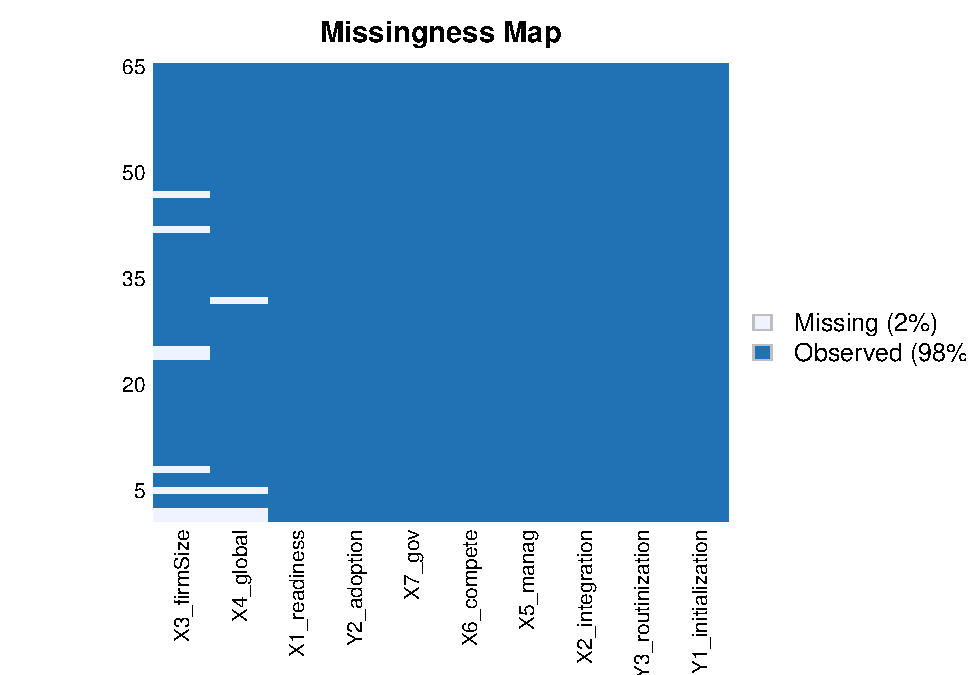
\includegraphics{markdown_report_files/figure-latex/unnamed-chunk-10-1.pdf}

\hypertarget{missing-value-imputation-in-amelia}{%
\subsubsection{Missing Value imputation in
Amelia}\label{missing-value-imputation-in-amelia}}

Here the log transformation has been applied to the X3\_firmSize since
the range for the firm size is too large, and a log transformation would
help to suppress the extreme large value of this variable.

\begin{Shaded}
\begin{Highlighting}[]
\KeywordTok{boxplot}\NormalTok{(TAA_data}\OperatorTok{$}\NormalTok{X3_firmSize, }\DataTypeTok{main=}\StringTok{"Boxplot for X3_firmSize"}\NormalTok{, }\DataTypeTok{horizontal=}\NormalTok{T)}
\end{Highlighting}
\end{Shaded}

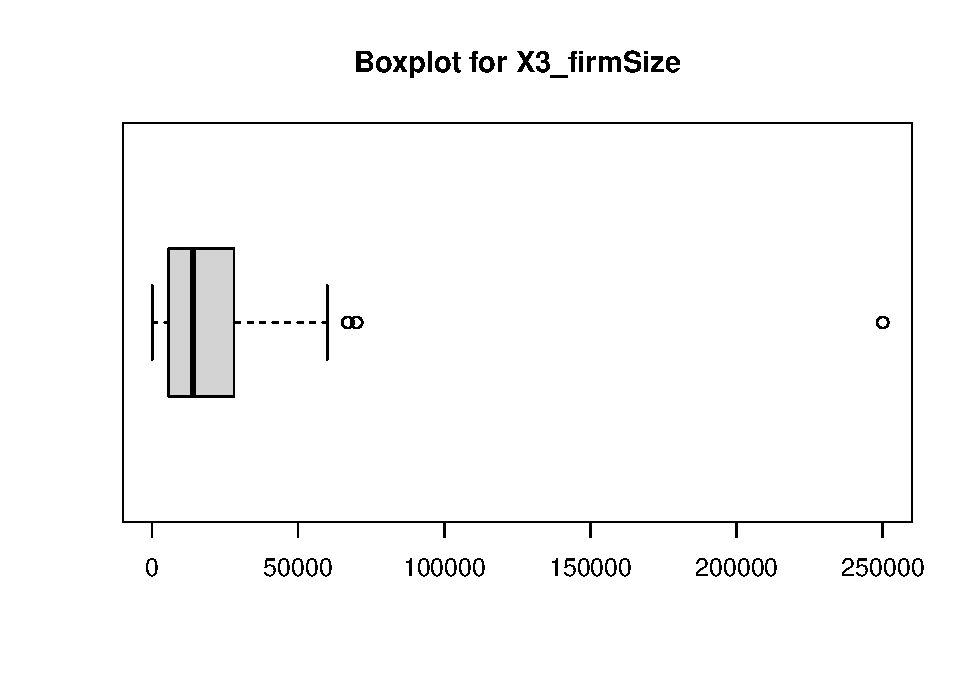
\includegraphics{markdown_report_files/figure-latex/unnamed-chunk-11-1.pdf}

Besides, since the global size is a categorical variable (nominal
variable), we want to specify this in the following function.

\begin{Shaded}
\begin{Highlighting}[]
\NormalTok{m =}\StringTok{ }\DecValTok{5} \CommentTok{# number of simulated datsets to create # See definition of m in ?amelia()}
\NormalTok{TAA_data_amelia <-}\StringTok{ }\KeywordTok{amelia}\NormalTok{(}\DataTypeTok{x =}\NormalTok{ TAA_data, }\DataTypeTok{logs=}\StringTok{"X3_firmSize"}\NormalTok{, }\DataTypeTok{noms=}\StringTok{"X4_global"}\NormalTok{, }\DataTypeTok{m =}\NormalTok{ m) }\CommentTok{# }
\end{Highlighting}
\end{Shaded}

\begin{verbatim}
## -- Imputation 1 --
## 
##   1  2  3  4  5  6  7  8  9 10 11
## 
## -- Imputation 2 --
## 
##   1  2  3  4  5  6  7  8
## 
## -- Imputation 3 --
## 
##   1  2  3  4  5  6
## 
## -- Imputation 4 --
## 
##   1  2  3  4  5  6  7
## 
## -- Imputation 5 --
## 
##   1  2  3  4  5
\end{verbatim}

\begin{Shaded}
\begin{Highlighting}[]
\KeywordTok{str}\NormalTok{(TAA_data_amelia}\OperatorTok{$}\NormalTok{imputations}\OperatorTok{$}\NormalTok{imp1)}
\end{Highlighting}
\end{Shaded}

\begin{verbatim}
## 'data.frame':    65 obs. of  10 variables:
##  $ X3_firmSize      : num  25000 28000 60000 15000 5600 26000 70000 16000 60000 20000 ...
##  $ Y1_initialization: num  0.578 0.646 0.251 0.185 0.513 ...
##  $ Y3_routinization : num  0.0819 -0.038 -0.9235 1.2726 -0.9235 ...
##  $ X2_integration   : num  -0.182 -0.758 -0.537 2.379 -0.758 ...
##  $ X5_manag         : num  0.0495 -0.4805 -0.1689 4.1609 -0.5452 ...
##  $ X6_compete       : num  -0.941 -0.941 -0.941 1.845 -0.941 ...
##  $ X7_gov           : num  1.633 0.753 -1.139 -1.43 1.563 ...
##  $ Y2_adoption      : num [1:65, 1] -0.492 0.205 -0.492 1.598 -1.188 ...
##  $ X1_readiness     : num [1:65, 1] 1.758 0.146 0.146 0.415 -1.197 ...
##  $ X4_global        : Factor w/ 2 levels "0","1": 2 2 2 2 2 2 2 2 2 2 ...
\end{verbatim}

\begin{Shaded}
\begin{Highlighting}[]
\NormalTok{TAA_data_impute <-}\StringTok{ }\NormalTok{TAA_data}
\CommentTok{# Average the imputations between different simulated datasets}
\NormalTok{col_index =}\StringTok{ }\KeywordTok{which}\NormalTok{(}\KeywordTok{names}\NormalTok{(TAA_data_amelia}\OperatorTok{$}\NormalTok{imputations}\OperatorTok{$}\NormalTok{imp1) }\OperatorTok\StringTok{ }\KeywordTok{c}\NormalTok{(}\StringTok{"X3_firmSize"}\NormalTok{, }\StringTok{"X4_global"}\NormalTok{))}
\ControlFlowTok{for}\NormalTok{( col }\ControlFlowTok{in}\NormalTok{ col_index)\{}
\NormalTok{  temp=}\KeywordTok{numeric}\NormalTok{()}
  \ControlFlowTok{for}\NormalTok{ (i }\ControlFlowTok{in} \DecValTok{1}\OperatorTok{:}\NormalTok{m)\{}
\NormalTok{    temp =}\StringTok{ }\KeywordTok{cbind}\NormalTok{(temp, TAA_data_amelia}\OperatorTok{$}\NormalTok{imputations[[i]][,col])}
\NormalTok{  \}}
\NormalTok{  TAA_data_impute[,col] =}\StringTok{ }\KeywordTok{apply}\NormalTok{(temp, }\DecValTok{1}\NormalTok{, mean)}
\NormalTok{\}}

\NormalTok{TAA_data_impute}\OperatorTok{$}\NormalTok{X4_global <-}\StringTok{ }\KeywordTok{round}\NormalTok{((TAA_data_impute}\OperatorTok{$}\NormalTok{X4_global))}
\end{Highlighting}
\end{Shaded}

\begin{Shaded}
\begin{Highlighting}[]
\KeywordTok{missmap}\NormalTok{(TAA_data_impute)}
\end{Highlighting}
\end{Shaded}

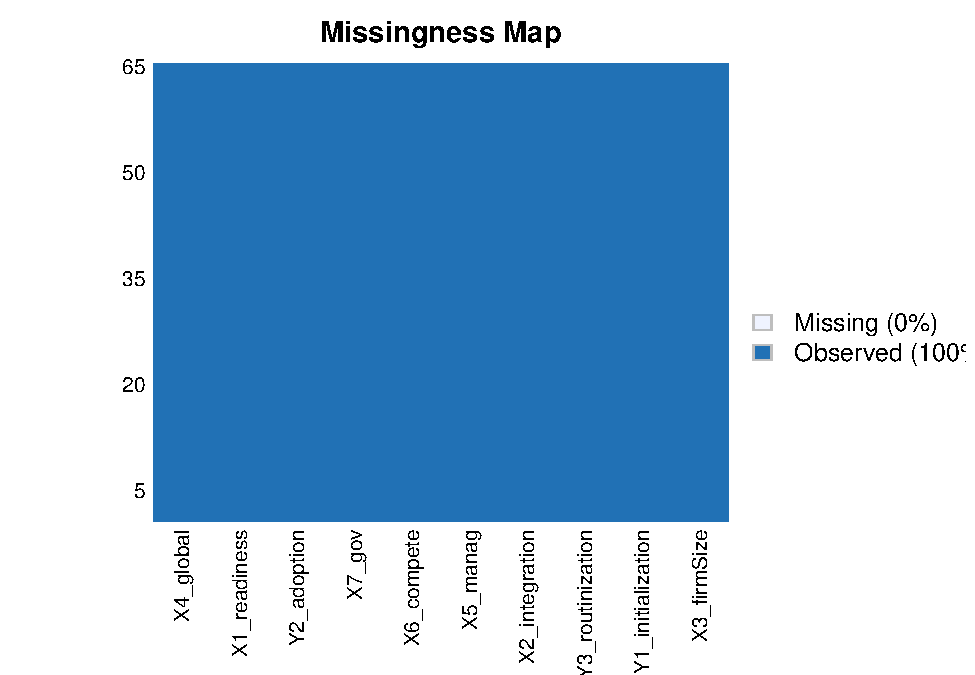
\includegraphics{markdown_report_files/figure-latex/unnamed-chunk-13-1.pdf}

Now we can see there are no missing values in the data set, and the
further regression analysis can be done.

Let's look at the summary of the missing value imputations.

\begin{Shaded}
\begin{Highlighting}[]
\KeywordTok{summary}\NormalTok{(TAA_data_impute)}
\end{Highlighting}
\end{Shaded}

\begin{verbatim}
##   X3_firmSize     Y1_initialization  Y3_routinization   X2_integration    
##  Min.   :    65   Min.   :-5.42871   Min.   :-1.41257   Min.   :-0.75756  
##  1st Qu.:  6586   1st Qu.:-0.05625   1st Qu.:-0.92351   1st Qu.:-0.75756  
##  Median : 14000   Median : 0.32550   Median : 0.05474   Median :-0.53722  
##  Mean   : 26253   Mean   : 0.01754   Mean   : 0.04283   Mean   :-0.02214  
##  3rd Qu.: 28000   3rd Qu.: 0.57846   3rd Qu.: 0.47586   3rd Qu.: 0.32497  
##  Max.   :250000   Max.   : 0.65275   Max.   : 4.12964   Max.   : 3.56297  
##     X5_manag          X6_compete             X7_gov        
##  Min.   :-0.86401   Min.   :-0.9413836   Min.   :-2.95425  
##  1st Qu.:-0.54522   1st Qu.:-0.9413823   1st Qu.:-0.57265  
##  Median :-0.26926   Median :-0.0580544   Median :-0.04600  
##  Mean   :-0.02177   Mean   : 0.0005798   Mean   : 0.02334  
##  3rd Qu.: 0.04952   3rd Qu.: 0.8776871   3rd Qu.: 0.75275  
##  Max.   : 4.16092   Max.   : 1.8450747   Max.   : 1.63342  
##     Y2_adoption.V1      X1_readiness.V1      X4_global    
##  Min.   :-1.1881243   Min.   :-1.1967245   Min.   :1.000  
##  1st Qu.:-0.4916377   1st Qu.:-0.9281527   1st Qu.:2.000  
##  Median :-0.4916377   Median :-0.1224372   Median :2.000  
##  Mean   : 0.0226910   Mean   :-0.0026128   Mean   :1.815  
##  3rd Qu.: 0.9013357   3rd Qu.: 0.6832784   3rd Qu.:2.000  
##  Max.   : 2.9907957   Max.   : 2.2947094   Max.   :2.000
\end{verbatim}

\begin{Shaded}
\begin{Highlighting}[]
\KeywordTok{par}\NormalTok{(}\DataTypeTok{mfrow=}\KeywordTok{c}\NormalTok{(}\DecValTok{2}\NormalTok{,}\DecValTok{1}\NormalTok{), }\DataTypeTok{mar=}\KeywordTok{c}\NormalTok{(}\DecValTok{2}\NormalTok{, }\DecValTok{3}\NormalTok{, }\DecValTok{2}\NormalTok{, }\DecValTok{3}\NormalTok{))}
\NormalTok{X4_orig <-}\StringTok{ }\KeywordTok{table}\NormalTok{(}\KeywordTok{as.character}\NormalTok{(TAA_data}\OperatorTok{$}\NormalTok{X4_global), }\DataTypeTok{useNA =} \StringTok{"ifany"}\NormalTok{)}
\NormalTok{X4_impute <-}\StringTok{ }\KeywordTok{c}\NormalTok{(}\KeywordTok{table}\NormalTok{(TAA_data_impute}\OperatorTok{$}\NormalTok{X4_global), }\DecValTok{0}\NormalTok{)}
\KeywordTok{rbind}\NormalTok{(X4_orig, X4_impute)}
\end{Highlighting}
\end{Shaded}

\begin{verbatim}
##            0  1 <NA>
## X4_orig   11 50    4
## X4_impute 12 53    0
\end{verbatim}

\begin{Shaded}
\begin{Highlighting}[]
\KeywordTok{par}\NormalTok{(}\DataTypeTok{mfrow=}\KeywordTok{c}\NormalTok{(}\DecValTok{2}\NormalTok{,}\DecValTok{1}\NormalTok{), }\DataTypeTok{mar=}\KeywordTok{c}\NormalTok{(}\DecValTok{2}\NormalTok{, }\DecValTok{3}\NormalTok{, }\DecValTok{2}\NormalTok{, }\DecValTok{3}\NormalTok{))}
\KeywordTok{compare.density}\NormalTok{(TAA_data_amelia, }\DataTypeTok{var=}\StringTok{"X3_firmSize"}\NormalTok{)}
\end{Highlighting}
\end{Shaded}

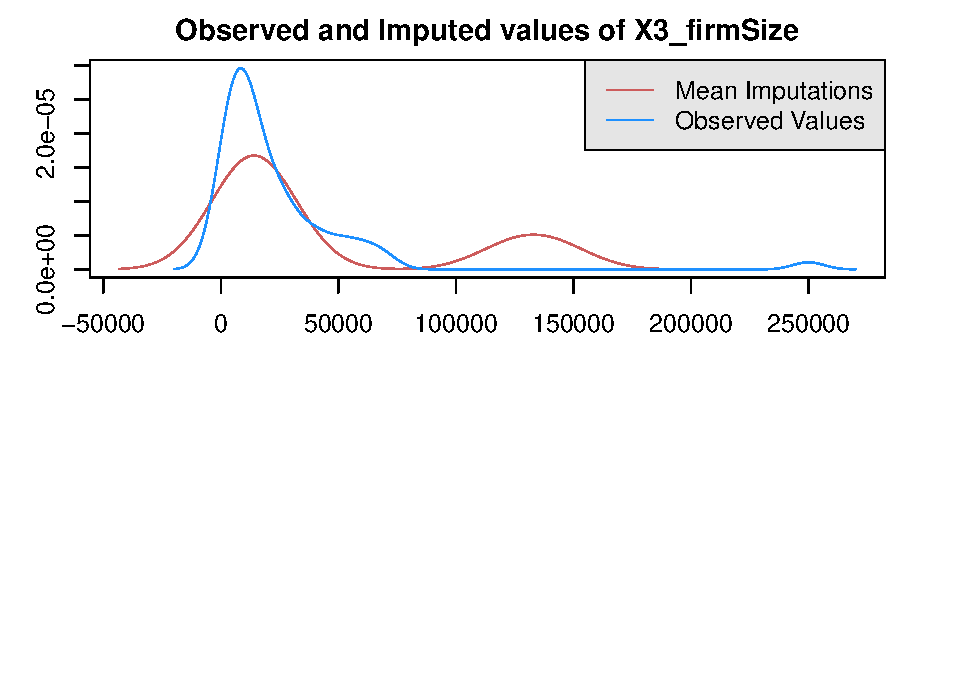
\includegraphics{markdown_report_files/figure-latex/unnamed-chunk-15-1.pdf}

Hence, the TAA\_data\_impute or TAA\_data\_scale can be applied to the
following analysis

\begin{Shaded}
\begin{Highlighting}[]
\CommentTok{# 1. log transformation of firmSize}
\NormalTok{TAA_data_impute}\OperatorTok{$}\NormalTok{X3_firmSize <-}\StringTok{ }\KeywordTok{log}\NormalTok{(TAA_data_impute}\OperatorTok{$}\NormalTok{X3_firmSize)}
\CommentTok{# 2. Make global a binary variable}
\NormalTok{TAA_data_impute}\OperatorTok{$}\NormalTok{X4_global <-}\StringTok{ }\KeywordTok{as.factor}\NormalTok{(TAA_data_impute}\OperatorTok{$}\NormalTok{X4_global)}
\CommentTok{# 2. scale of data}
\NormalTok{TAA_data_scale =}\StringTok{ }\KeywordTok{cbind}\NormalTok{(}\KeywordTok{scale}\NormalTok{(TAA_data_impute[,}\DecValTok{1}\OperatorTok{:}\DecValTok{9}\NormalTok{]),TAA_data_impute[,}\DecValTok{10}\NormalTok{])}
\KeywordTok{colnames}\NormalTok{(TAA_data_scale)[}\DecValTok{10}\NormalTok{]=}\StringTok{"X4_global"}
\KeywordTok{str}\NormalTok{(TAA_data_scale)}
\end{Highlighting}
\end{Shaded}

\begin{verbatim}
##  num [1:65, 1:10] 0.49 0.575 1.146 0.107 -0.632 ...
##  - attr(*, "dimnames")=List of 2
##   ..$ : chr [1:65] "3" "4" "6" "7" ...
##   ..$ : chr [1:10] "X3_firmSize" "Y1_initialization" "Y3_routinization" "X2_integration" ...
\end{verbatim}

\hypertarget{multivariate-regression-analysis-qiang}{%
\subsubsection{Multivariate Regression Analysis
(Qiang)}\label{multivariate-regression-analysis-qiang}}

\hypertarget{regression-trees-drew}{%
\subsubsection*{Regression Trees (Drew)}\label{regression-trees-drew}}
\addcontentsline{toc}{subsubsection}{Regression Trees (Drew)}

\hypertarget{refs}{}
\leavevmode\hypertarget{ref-linting2007nonlinear}{}%
Linting, Mariëlle, Jacqueline J Meulman, Patrick JF Groenen, and Anita J
van der Koojj. 2007. ``Nonlinear Principal Components Analysis:
Introduction and Application.'' \emph{Psychological Methods} 12 (3):
336.

\end{document}
